\documentclass{article}
\usepackage{tikz, comment}
\usepackage{pifont}
\usepackage{fontspec}
\usetikzlibrary{arrows, decorations.markings, decorations.pathreplacing}
\begin{comment}
:Title: Not defined yet
:Tags: focus of a parabola;directrix of a parabola;parabola;moment;focal radius 
:Prob: 0.5742;0.5723;0.5651;0.4694;0.4689
:Author: Prof.Hu Ji-shan, HKUST
:Slug: No name yet

Description Here.........
\end{comment}
\begin{document}\centering

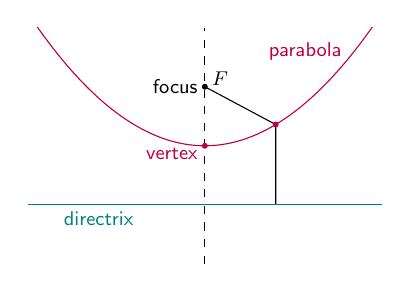
\begin{tikzpicture}[>=latex,xscale=.5*1.5, yscale=.5*1.5][font=\sf\small]

\coordinate (F) at (0, 1);
\coordinate (P) at (1.2, {1/4*1.2^2});
\coordinate (Q) at (1.2, -1);

\clip[] (-3,-2) rectangle (3,2);

\draw[dashed] (0, -2) -- (0, 2);

\draw (F)--(P)--(Q);
\tkzMarkSegment[color=blue,pos=.5,mark=||](F,P);
\tkzMarkSegment[color=blue,pos=.5,mark=||](P,Q);

\draw[purple, samples=100, smooth, domain=-3:3, variable=\x]
plot ({\x}, {1/4*(\x)^2}) ;

\draw[teal] (-3,-1) -- (3, -1) node[below, pos=0.2, scale=0.8]{$\hbox{directrix}$};

\draw[fill, xscale=1/1.5, yscale=1/1.5] (0, 1*1.5) circle(0.06) node[left, scale=0.8]{$\hbox{focus}$} node[right, yshift=3, scale=0.8]{$F$};

\draw[purple, fill, xscale=1/1.5, yscale=1/1.5] (P) circle(0.06);
\draw[purple, fill, xscale=1/1.5, yscale=1/1.5] (0, 0) circle(0.06)node[left, yshift=-3, scale=0.8]{$\hbox{vertex}$};

\node[purple, scale=0.8] at (1.7, 1.6) {$\hbox{parabola}$};

\end{tikzpicture}
\end{document}